% Metódy inžinierskej práce

\documentclass[10pt,slovak,a4paper]{article}

\usepackage[slovak]{babel}
\usepackage[T1]{fontenc}
\usepackage[IL2]{fontenc} 
\usepackage[utf8]{inputenc}
\usepackage{graphicx}
\usepackage{booktabs}
\usepackage{enumitem}
\usepackage{pgfplots}
\usepackage{url} 
\usepackage{hyperref} 
\usepackage{cite}
\pagestyle{headings}
\graphicspath{{subory}}

\title{Spracovanie jazyka pri inteligentnom hlasovom vyhľadávaní\thanks{Semestrálny projekt v predmete Metódy inžinierskej práce, ak. rok 2023/24, vedenie: Ing. Mohammad Yusuf Momand, MSc.}} % meno a priezvisko vyučujúceho na cvičeniach

\author{Martin Kvietok\\[2pt]
	{\small Slovenská technická univerzita v Bratislave}\\
	{\small Fakulta informatiky a informačných technológií}\\
	{\small \texttt{xkvietokm@stuba.sk}}
	}
\date{\small 30. november 2023} 

\begin{document}
\maketitle
\begin{abstract}

V súčasnosti zohráva spracovanie jazyka (NLP) veľmi dôležitú úlohu pri efektívnom vyhľadávaní informácií na intrenete. Bežným postupom ako niečo vyhľadať je napísanie výrazu na klávesnici. No s dnešnými modernými technológiami vieme vyhľadať potrebný výraz ešte ľahšie a dokonca bez písania. Takéto riešenie výrazne urýchľuje proces práce s informáciami a ušetrí používateľom veľa času. V tejto práci predstvím použiteľnosť tohto riešenia , inovatívne vyhľadávanie hlasom pomocou Smart Voice Search Engine (SVSE)
, ktorého základ tvorí spracovanie prirodzeného jazyka. NLP umožňuje počítačom porozumieť ľudskému jazyku, čo je kľúčovým prvkom aktuálnej problematiky. V tejto práci sa ďalej budem snažiť detailnejšie vysvetliť princíp fungovania NLP a jeho implementáciu v rámci SVSE, taktiež funkciu rozpoznávania hlasu používateľa a praktickú využiteľnosť v budúcich projektoch.
\end{abstract}

\section{Úvod}
V dnešnej dobe je prístup k informáciám a službám na internete takmer samozrejmý, pričom hovorené slovo sa stáva prirodzeným nástrojom na vyhľadávanie a pomaly nahrádza nepraktické písanie na klávesnici. V uplynulých desaťročiach sme boli svedkami prudkého vývoja v oblasti rozpoznávania prirodzeného jazyka. To malo za následok, že už v roku 2007 dosiahla firma Google prelomové výsledky, keď rozšírila aplikáciu Google Maps o funkciu hlasového vyhľadávania. Tento vývoj následne viedol k vzniku personalizovaných hlasových asistentov, ktorí sú schopní okamžite vyhľadávať informácie na základe hovorených otázok a efektívne transformovať reč na užitočný obsah. Tento článok sa zaoberá problematikou rozpoznávania jednotlivých používateľov a ich konkrétnej reči. Taktiež uvádza komplexný model s označením SVSE, ktorý je navrhnutý s cieľom zvýšiť dostupnosť a efektivitu hlasového vyhľadávania na internete.

\section{Spracovanie prirodzeného jazyka (NLP)} 
Spracovanie prirodzeného jazyka (NLP) je odvetvie informatiky, ktoré sa zaoberá vytváraním počítačových systémov schopných pracovať s ľudským jazykom. Začiatky spracovania prirodzeného jazyka (NLP) sa datujú približne od roku 1950 \cite{TechTarget:NLP}, no od tej doby prechádza NLP neustálym vývojom, ktorý pokračuje až po súčasnosť. Každý rok so sebou prináša stále nové a fascinujúce možnosti.
Jeden z najvýraznejších momentov bol dosiahnutý modelom GPT-3 (Generative Pre-trained Transformer 3) od spoločnosti OpenAI už v roku 2022. GPT-3 je najväčší a najvýkonnejší jazykový model schopný produkovať pôsobivý a gramaticky správny text, odpovedať na otázky, a dokonca vytvárať kreatívne textové obsahy. Celý príncíp fungovania je založnený na procesoch porozumenia a generovania prirodzeného jazyka.
\begin{figure}[h]
  \centering
  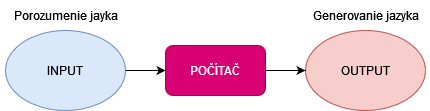
\includegraphics[width=10cm]{NLP.png}
  \caption{Diagram 1: Princíp NLP}
  \cite{sarhan2014smart}
\end{figure}

\leavevmode \newline
"Porozumenie jazyka (NLU) je akýmsi jazykovým detektívom, ktorý zisťuje význam slov v texte, zatiaľ čo Generovanie jazyka (NLG) je kováčom, ktorý formuje slová zrozumiteľné pre počítače."
\newline
\newline
Vstupný text vždy prechádza 5 alnalýzami, počas ktorých sa kontroluje.
\begin{enumerate}
    \item\textbf{Rozdelenie textu na slová a vety} 
    \item\textbf{Gramatické štruktúra vety}
    \item\textbf{Význam slova z kontextu}
    \item\textbf{Vzájomná závislosť viet} 
    \item\textbf{Správna interpretácia}
\end{enumerate}
\cite{builtin-nlp-intro}
\leavemode\newline
Pri identifikácii jazyka zohráva kľúčovú úlohu predovšetkým strojové učenie (Machine Learning). V minulosti sa identifikácia jazyka zakladala na množstve pravidiel a výnimiek (if-else), čo robilo tento proces časovo neefektívnym a nepraktickým. Strojové učenie je založené na automatickom získavaní a používaní informácií prostredníctvom analýzy príkladov z reálneho sveta. Tieto algoritmy využívajú ako vstupný zdroj veľké množstvo dát a to v praxi znamená - čím viac dát je k dispozícii, tým má daný algoritmus menšiu mieru chybovosti. Systémy založené na algoritmoch strojového učenia majú mnohé výhody oproti ručne vytvoreným pravidlám. 
\cite{chopra2013natural}

\section{Koncept SVSE} \label{ina}
Prvé využitie vyhľadávania hlasom bolo uvedené na trh už v roku 2008 v alpikácii Google Mobile App pre iPhone. Táto funkcia rozšírila možnosti hlasového vyhľadávania zo skôr obmedzeného vyhľadávania podnikov na mapách na neobmedzené vyhľadávanie po celom internete. Vyhľadánie na Google hlasom musí byť schopné spracovať všetko, čo dokážu aj bežné internetové prehlidače. To z neho robí pomerne náročný rozpoznávací systém, pretože slovná zásoba a komplexnosť otázok sú veľmi veľké. 
\cite{schalkwyk2010your}

\subsection{Princíp Rozpoznania Hlasu Používateľa} 
Proces rozpoznávania hlasu užívateľa sa skladá z 3 dôležitých aspektov.
\begin{enumerate}
    \item\textbf{Indentifikácia} - je proces určenia, od ktorého z registrovaných rečníkov pochádza daný prejav
    \item\textbf{Overenie} - je proces prijatia alebo odmietnutia identifikácie
       \item\textbf{Diarizácia} - je proces odelenia reči v prípade rozprávania viacerých užívateľov súčastne

  \begin{figure}[h]
    \centering
    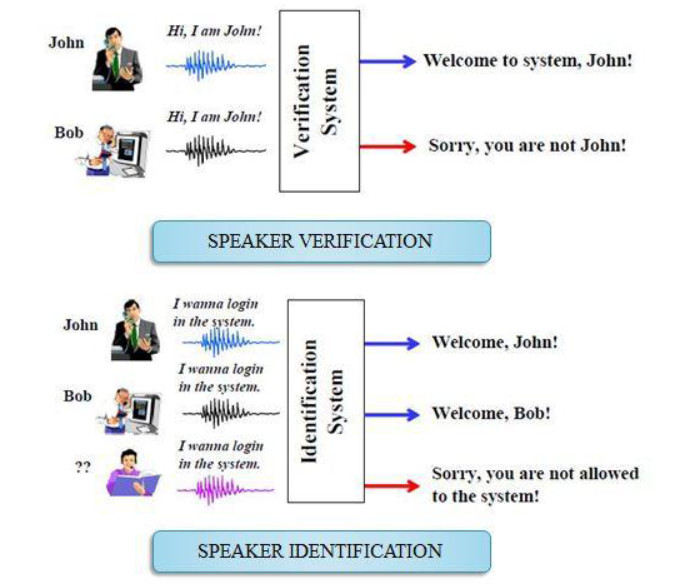
\includegraphics[width=10cm]{speaker.png}
    \caption{Identifikácia a overenie používateľa}
    \cite{speakerrecognitionthesis}
  \end{figure}
\leavevmode \newline
\leavevmode \newline
\leavevmode \newline
\leavevmode \newline

\subsection{Model SVSE} \label{ina:este}
Základné parametre s ktorými SVSE pracuje.
\begin{itemize}
    \item\textbf{Word Error Rate} (miera chýb,UX vs SVSE) 
    \item\textbf{WebScore}(optimalizácia chýb UX)
    \item\textbf{Perplexity} (predpoveď vstupu UX)
    \item\textbf{Out-of-Vocabulary Rate} (rozpoznanie jazyka UX)
    \item\textbf{Latency} (celkový čas vyhľadávania)
\end{itemize}
\cite{schalkwyk2010your}

\subsection{Princíp vyhľadávania}\label{ina}
\leavemode\newline
Pred samotným vyhľadávaním je nevyhnutné digitalizovať zvuk pomocou analógovo-digitálneho konvertora. Tým sa akustický zvuk z mikrofónu prevedie do digitálnej podoby. Tento digitálny formát sa ďalej analyzuje a vizualizuje vo forme spektrogramu, ktorý podáva detailné informácie o frekvencii, intenzite a časovej štruktúre zvukového záznamu.
\leavevmode \newline
\leavevmode \newline
Následne pre lepšie pochopenie a spracovanie textu sa využijú pokročilé metódy, ako je Hidden Markov Model (HMM) alebo Neurónové Siete, ktoré sú zamerané na prácu s fonémami (základnými jednotkami reči).
\leavevmode \newline
\leavevmode \newline
Nakoniec je potrebné prejsť procesom normalizácie textu, ktorý transformuje písanný textu do jeho štandardizovanej formy. Pri vytváraní jazykových modelov, napríklad pre vyhľadávanie pomocou hlasu, je dôležité dosiahnuť konzistentnú a zrozumiteľnú reprezentáciu dopytov nezávisle na ich pôvodnej podobe. Uvediem príklad na pôvodnú podobu dopytu:
\newline
\newline
\textbf{"Koľko je teraz hodín v Bratislave?"}	
\newline
\newline
Podobne ako v predchádzajúcom príklade, konzistentná a zrozumiteľná reprezentácia dopytu by zahŕňala aj iné možné formulácie ako napríklad:
\begin{enumerate}[label=\Roman*.]
  \item\textbf{"Aký je aktuálny čas v Bratislave?"}
  \item\textbf{"Povedz mi prosím, koľko je hodín v Bratislave?"}
  \item\textbf{"V Bratislave je teraz koľko hodín?"}
\end{enumerate}   
Aby jazykový model rozumel týmto formuláciám otázok a bol schopný na ne adekvátne reagovať, je potrebné ich všetky zaradiť do reprezentácie pre dopyt ohľadom aktuálneho času v Bratislave.
Hlavným cieľom je zjednodušiť text pre ďalšiu analýzu alebo spracovanie. 
Medzi metódy normalizácie patrí odstránenie diakritiky, tokenizácia (rozdelenie textu na jednotlivé slová alebo vety), odstránenie interpunkcie, konverzia slov do ich základných tvarov a rozvoj skratiek. Významnou časťou normalizácie sú procesy ako stemming a lemmatizácia. 
\leavevmode \newline
\leavevmode \newline
Proces tokenizácie textu na príklade:
\leavevmode \newline
\textbf{['Koľko', 'je', 'teraz', 'hodín', 'v', 'Bratislave']}
\leavevmode \newline
\leavevmode \newline
Stemming sa snaží redukovať slová na ich koreňový tvar, často nezávisle na tom, či výsledný tvar je platné slovo v slovníku.
\leavevmode \newline
Ukážka stemmingu na príklade:
\leavevmode \newline
\textbf{['koľko', 'je', 'teraz', 'hodín', 'v', 'bratislav']}
\leavevmode \newline
\leavevmode \newline
Naopak, lemmatizácia sa snaží slová redukovať na základný tvar, ktorý je platným slovom v danej jazykovej sústave.
\leavevmode \newline
Ukážka lemmatizácie na príklade:
\leavevmode \newline
\textbf{['Koľko', 'je', 'teraz', 'hodín', 'v', 'Bratislava']}
\leavevmode \newline
\leavevmode \newline
Tieto techniky normalizácie majú za cieľ zjednodušiť text a urobiť ho vhodným pre ďalšiu analýzu a spracovanie v rámci aplikácií spracovania prirodzeného jazyka (NLP) a podobných oblastí.\cite{lopezyse2021}
\leavevmode \newline
\leavevmode \newline
Vo finálnom kroku bude postupne skúmaná sekvencia slov, ktorá bola identifikovaná. Tieto slová budú použité na vyhľadanie informácií na Google. Výsledky vyhľadávania budú overované, aby sa zistilo, či presne zodpovedajú tomu, čo používateľ hľadá. Ak nie, systém sa pozrie na inú možnosť sekvencie slov a pokračuje v tomto procese, kým nenájde tú správnu. Potom systém zaznie signál, aby používateľa informoval o výsledkoch.
\cite{schalkwyk2010your}

\section{Efektívnosť} 
\begin{table}[h]
    \centering
    \begin{center}
        \begin{tabular}{lccc}
            \toprule
            \textbf{Rozhovor(min)} & \textbf{Počet hovoriacich} & \textbf{Pohlavie} & \textbf{Presnosť rozpoznania} \\
            \midrule
            Do 10 & 2 & Muž/Žena/Mix & 65\%/62\%/71\% \\
            Do 10 & 5 & Muž/Žena/Mix & 55\%/51\%/65\% \\
            Nad 10 & 2 & Muž/Žena/Mix & 69\%/67\%/74\% \\
            Nad 10 & 5 & Muž/Žena/Mix & 60\%/55\%/69\% \\
            \bottomrule
        \end{tabular}
    \end{center}
    \caption{Tabuľka testov SVSE}
    \label{tab:mytable}
    \cite{sarhan2014smart}
\end{table}

\leavevmode \newline
Efektívnosť SVSE spočíva predovšetkým v presnom rozpoznávaní používateľa a správnom porozumení hľadaného textu. Počas testov zameraných na rozpoznávanie používateľov sa systému podarilo dosiahnuť presnosť vyššiu ako 50\% u každého rečníka. Najlepšie výsledky boli zaznamenané pri dlhších rozhovoroch medzi mužom a ženou.

Tento úspech môže byť pripisovaný implementácii strojového učenia. Systém sa dokázal prispôsobiť rôznorodej slovnej zásobe a výrazom používateľov. Kľúčovým faktorom bolo, že systém je schopný lepšie porozumieť a rozpoznať rečníka, keď má k dispozícii viac vzorových údajov. 

V dnešnej dobe je teda stále kľúčové investovať do zbierania a analýzy vzorových údajov a ich následné využitie pri vylepšovaní schopností hlasových vyhľadávačov. Týmto spôsobom môžu tieto systémy lepšie zodpovedať potrebám používateľov a ponúkať im personalizovaný a efektívny zážitok pri interakcii s technológiou.
\cite{masterofcode-voice-assistants}

\section{Potencionálne nedostatky} 
\begin{enumerate}
    \item\textbf{Neznámy jazykový vstup} - Algoritmy rozpoznávania hlasu môžu rozumieť iba naučeným jazykom, dialektom a prízvukom.
    \item\textbf{Ochrana súkromia} - Tieto zariadenia  zbierajú a uchovávajú informácie o tom, čo používatelia vyhľadávali a ukladajú ich hlasové záznamy. Na zmiernenie niektorých obáv je dnes hlasový údaj klasifikovaný ako biometrická informácia a chránený všetkými hlavnými zákonmi o súkromí. Firmy, ktoré chcú využívať túto technológiu, musia dodržiavať striktné predpisy.
    \cite{luigisbox-voice-search-optimization}
    \leavevmode 
    \item\textbf{SEO} - Prvé zobrazované výsledky vyhľadávania majú vždy najvyššiu prioritu. Algoritmus prehliadne nižšie hodnotené webové stránky, čo znamená, že potenciálni zákazníci sa o nich nikdy nedozvedia.
    \cite{victoriousseo_voice_search}
\end{enumerate}}
\leavevmode \newline

\section{Budúcnosť hlasových vyhľadávačov}
Graf používania hlasových vyhľadávačov jasne ukazuje, že sa hlasovo-ovládné technológie rýchlo stávajú neoddeliteľnou súčasťou každodenného života ľudí. Táto zmena v správaní a preferenciách používateľov bezpochyby súvisí s výhodami, ktoré hlasové vyhľadávanie prináša. Pohodlie a rýchlosť, charakteristické pre túto formu interakcie, vytvárajú prostredie, v ktorom je hlasové vyhľadávanie vnímané ako efektívny a prirodzený spôsob získavania informácií.
\cite{Smith2022}

\begin{figure}[t]
    \centering
    \begin{tikzpicture}
        \begin{axis}[
            title={Number of Voice Assistant Users (2017-2023)},
            xlabel={Year} \cite{demandsage2023},
            ylabel={Number of Users (in millions)},
            ybar,
            symbolic x coords={2017,2018,2019,2020,2021,2022,2023},
            xtick=data,
            nodes near coords,
            nodes near coords align={vertical},
        ]
        \addplot coordinates {
            (2017, 79.9)
            (2018, 103.9)
            (2019, 115.2)
            (2020, 128)
            (2021, 132)
            (2022, 123.5)
            (2023, 125.2)
        };
        \end{axis}
    \end{tikzpicture}
\end{figure}

\leavevmode \newline
\leavevmode \newline
\leavevmode \newline\leavevmode \newline
\leavevmode \newline
\leavevmode \newline\leavevmode \newline
\leavevmode \newline
\leavevmode \newline\leavevmode \newline
\leavevmode \newline
\leavevmode \newline
\leavevmode \newline
\label{fig:voice_assistant_users}
\paragraph{Historické súvislosti.}Aj v oblasti informatiky nájdeme plno fascinujúcich osobností, ktoré zanechali za sebou nezmazateľnú stopu v histórii ľudstva a ktorých výsledky prác používame dodnes. Existovali by vôbec počítače keby nebolo 7 statočných inžinierov? Gottfried Wilhelm Leibnitz, ktorý priniesol ideu zápisu čísel do binárnej sústavy. George Boole zakladateľ Booleovskej algebry a logiky. Gottlog Frege s jeho  prvým symbolického jazykom založeného na matematike a logike. Taktiež Cantor, Hilbert a Gödel , ktorí svojimi príspevkami položili základy informatiky prostredníctvom pokrokov v teórii množín, matematickej logike a pochopení výpočtových limitov. A nakoniec Alan Turing vynálezca Univerzálneho stroja, dnes označovaný ako počítač (stroj používaný na viac nezávislých činností). Nanešťastie, žiadny z týchto pánov už dnes nie je medzi nami, avšak výsledky ich práce budú ovplyvňovať naše každodenné životy ešte dlhú dobu.   
\paragraph{Technológia a ľudia.} Projekt = premietnutie idey do reality. Pred začatím každého projektu je potrebné všetko detailne premyslieť a zdokumentovať. Následne by sme mali konať v iteráciách v poradí 1.Špecifikácia 2.Návrh 3.Implementácia. Dôležité je dodržiavať stanovený plán a venovať sa prioritám. Efektívna metóda pre prácu v tíme je využitie SCRUMu. Scrum je jednoduchý spôsob riadenia projektov, kde tímy pracujú spoločne na malých kúskoch produktu, stretávajú sa denne na krátkom stretnutí na prehodnocujú svoje ciele. Týmto spôsobom poskytujeme tímu jasný rámec na plánovanie a sledovanie práce.
\paragraph{Udržateľnosť a etika.} Rozvoj = postupný rast, rozširovanie, zdokonaľovanie. Pre spoločnosť vplýva pozitívne a je potrebný pri každej práci, vrátane inžinierov. Prináša nám nové objavy a cesty do budúcnosti, avšak čelíme aj mnohým výzvam ako vyčerpávanie prírodných zdrojov alebo nadmerná produkcia odpadu. Tieto problémy si vyžadujú inovatívne riešenia v podobe tzv. udržateľného rozvoju (rozvoj, ktorý berie ohľad na budúcnosť, nie iba na aktuálny stav) Etika = vo vzťahu ku kultúre a globálnej spoločnosti, v práci a podnikaní rovnako v informačných technológiách. Etika má aj svoje regulácie, ktoré bývajú najčastejšie spísané v kódexoch pre určité zamerania, ku príkladu medici majú Hippokratova prísaha, IEEE je pre profesijné združenia a Software Engineering Code of Ethics využívame v informačných technológiách. 

\section{Záver} \label{zaver}
Spracovanie jazyka je nevyhnutnou súčasťou inteligentného hlasového vyhľadávania, ktoré sa stáva čoraz populárnejším prostriedkom interakcie medzi človekom a technológiou. Táto technológia umožňuje užívateľom komunikovať so zariadeniami a aplikáciami prirodzenejším spôsobom prostredníctvom hlasu. Efektívnosť vyhľadávačov sa každým rokom zlepšuje aj vďaka postupnému nasadzovaniu algoritmov strojového a hĺbkového učenia. No predsa tu môžeme nájsť pár nedostatkov, ktoré je potrebne do budúcnosti vyriešiť. Celkový proces získavania informácii z hlasového vstupu a následné porovnávanie pomocou vyhľadávača prestavuje súbor komplexných procesov, ktorý som sa snažil v tejto práci zjednodušene spracovať. 
Celkovo je však jasné, že spracovanie jazyka hrá kľúčovú úlohu v rozvoji inteligentného hlasového vyhľadávania a prispieva k vytváraniu užívateľsky príjemnejších a efektívnejších interakcií s technológiou prostredníctvom hlasu.

\bibliography{literatura}
\bibliographystyle{plain} 
\end{document}
